% !TeX root = probability.tex

%%%%%%%%%%%%%%%%%%%%%%%%%%%%%%%%%%%%%%%%%%%%%%%%%%%%%%%%%%%%%%

\section{קיץ תשפ"א מועד ב}

\begin{center}
\selectlanguage{english}
\includegraphics[width=\textwidth]{summer-2021b-3}
\end{center}

נניח שההסתברויות לעבור כל מכשול בלתי-תלויות. נסמן ב-%
$M1, M2, M3$ \L{(mikhshol)}
את המאורעות של לעבור כל מכשול, ונסמן ב-%
$HG$ \L{(hatzi gmar)}
את המאורע לעלות לחצי הגמר.

\textbf{סעיף א}

לפי ההנחה שהצלחה לעבור מכשול בלתי תלוי במכשולים האחרים, ההסתברות לעבור סדרה של מכשולים היא המכפלה של ההסתברויות של המכשולים. נתון ש-%
$P(M1)P(M2)=0.28$.
אם משתתף עבר את שני המכשולים הראשונים, ההסתברות שהוא יעלה לחצי הגמר שווה להתסתברות שהוא יעבור את המכשול השלישי:
\begin{eqn}
P(M3)&=&3(1-P(M3))\\
P(M3)&=&0.25\\
P(HG)&=&P(M1)P(M2)P(M3)=0.28\cdot 0.25=0.07\,.
\end{eqn}

\textbf{סעיף ב}

נתון
$P(M1)P(\overline{M2})=0.42$
ולפי הסתברות שלמה:
\begin{eqn}
P(M1)&=&P(M1)P(M2)+P(M1)P(\overline{M2})=0.28+0.42=0.70\\
P(\overline{M1})&=&1-P(M1)=0.30\,.
\end{eqn}

\textbf{סעיף ג 1}

ההסתברות של משתתף אחד לעלות לחצי הגמר היא:
\[
P(HG/M1)=\frac{P(HG\cap M1)}{P(M1)}=\frac{P(HG)}{P(M1)}=
\frac{0.07}{0.70}=0.01\,,
\]
כאשר אנו משתמשים ב-%
$HG \subseteq M1$
כי משתתף עולה לחצי הגמר רק אם הוא עבר את כל המכשולים, קל וחומר  את המכשול הראשון.

המילה "בדיוק" מכוונת לנוסחת ברנולי, לכן ההסתברות המבוקשת היא:
\[
{3\choose 2}\left(0.01\right)^2\left(0.90\right)^1=0.027\,.
\]

\textbf{סעיף ג 2}

נסמן ב-%
$O,G,L$
את המאורעות שעומר, גל וליאור יעלו לחצי הגמר. נניח כרגיל שההצלחות של המשתתפים בלתי-תלויות:
\[
P(O)P(G)P(\overline{L}) =
\left(0.10\right)\left(0.90\right)\left(0.10\right)=0.009\,.
\]

%%%%%%%%%%%%%%%%%%%%%%%%%%%%%%%%%%%%%%%%%%%%%%%%%%%%%%%%%%%%%

\newpage

\section{קיץ תשפ"א מועד א}

\begin{center}
\selectlanguage{english}
\includegraphics[width=\textwidth]{summer-2021a-3}
\end{center}

הפסקאות "מן המורים" ו-"מכלל המשתתפים" אינן מכוונות להסתברות מותנית, כי הן מתייחסות לכל הקבוצה של המורים וכל הקבוצה של המשתתפים. הפסיק ב-"מכלל המשתתפים (מורים ותלמידים), שנבדקו לגילוי קורונה" מבלבל כי אפשר לפרש שהנתון הוא
$13/15$
"מכלל המשתתפים בסקר".

נסמן ב-%
$M$ \L{(moreh)}
את המאורע של מורה שנסקר בסקר, ואז
$\overline{M}$
הוא המאורע של תלמיד שנסקר בסקר. נסמן ב-%
$N$ \L{(nivdak)}
את המאורע של נבדק לקורונה.

\textbf{סעיף א}

יש שני סוגים של מאורעות ולכן הארגן את המידע בטבלה. 

תחילה נחשב:
\begin{eqn}
P(\overline{M})&=&1-P(M)=9P(M)\\
P(M)&=&0.10\,.
\end{eqn}
נתון ש:
\[
P(N/M)=\frac{P(N\cap M)}{P(M)}=0.80\,,
\]
ולכן:
\[
P(N\cap M) = 0.80P(M)=0.08\,.
\]
את התוצאות הללו נכניס לתאים בטבלה תוך הוספת הסתברויות משלימות:
\begin{center}
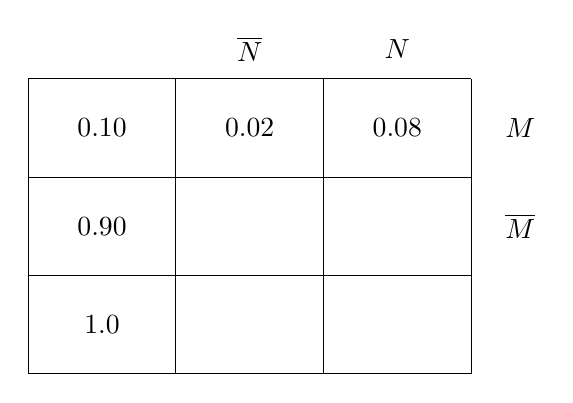
\begin{tikzpicture}[scale=1.25]
\draw (0,0) grid[xstep=1.5] (4.5,3);
\node at (3.75,3.3) {$N$};
\node at (2.25,3.3) {$\overline{N}$};
\node at (5,2.5) {$M$};
\node at (5,1.5) {$\overline{M}$};

\node at (3.75,2.5) {$0.08$};
\node at (2.25,2.5) {$0.02$};
\node at (0.75,2.5) {$0.10$};

\node at (3.75,1.5) {$$};
\node at (2.25,1.5) {$$};
\node at (0.75,1.5) {$0.90$};

\node at (0.75,0.5) {$1.0$};
\node at (2.25,0.5) {$$};
\node at (3.75,0.5) {$$};
\end{tikzpicture}
\end{center}
נתון נוסף הוא:
\[
P(\overline{M}/N)=\frac{P(\overline{M}\cap N)}{P(N)}=\frac{13}{15}\,.
\]
נשתמש בהסתברויות משלימות ונקבל:
\begin{eqn}
P(N)&=&P(M\cap N)+P(\overline{M}\cap N)\\[6pt]
&=&0.08+\frac{13}{15}P(N)\\
P(N)&=&0.60\,.
\end{eqn}
נמלא את שאר התאים בטבלה ונמצא את התשובה:
\[
P(\overline{M}\cap \overline{N})=0.38\,.
\]
\begin{center}
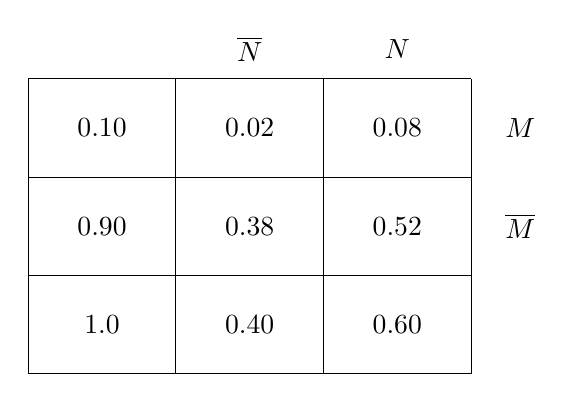
\begin{tikzpicture}[scale=1.25]
\draw (0,0) grid[xstep=1.5] (4.5,3);
\node at (3.75,3.3) {$N$};
\node at (2.25,3.3) {$\overline{N}$};
\node at (5,2.5) {$M$};
\node at (5,1.5) {$\overline{M}$};

\node at (3.75,2.5) {$0.08$};
\node at (2.25,2.5) {$0.02$};
\node at (0.75,2.5) {$0.10$};

\node at (3.75,1.5) {$0.52$};
\node at (2.25,1.5) {$0.38$};
\node at (0.75,1.5) {$0.90$};

\node at (0.75,0.5) {$1.0$};
\node at (2.25,0.5) {$0.40$};
\node at (3.75,0.5) {$0.60$};
\end{tikzpicture}
\end{center}

\textbf{סעיף ב}

הניסוח "בזה אחר זה" מכוון להתפלגות בינומית. נקצר את הסימון 
$P(N)$
ל-%
$p$
ולפי סעיף א 
$p=0.60$.
לפחות ארבעה משתתפים שקול לארבעה או חמישה משתתפים:
\begin{eqn}
P(N\geq 4) &=& {5 \choose 4}p^4(1-p)^1+{5 \choose 5}p^5(1-p)^0\\
&=& 5\cdot 0.60^4\cdot 0.40 + 0.60^5=0.3370\,.
\end{eqn}

\textbf{סעיף ג}

המילה "ידוע" מכוון להסתברות מותנית. ברור ש-%
$N\geq 4\subseteq N\geq 1$
ולכן:
\begin{eqn}
P(N\geq 4 / N\geq 1)&=&\frac{P((N\geq 4) \cap (N\geq 1))}{P(N\geq 1)}=\frac{P(N\geq 4)}{P(N\geq 1)}=\frac{P(N\geq 4)}{1-P(N=0)}\\[6pt]
&=& \frac{0.3370}{1-(1-p)^5}=\frac{0.3370}{0.9898}=0.3404\,.
\end{eqn}

\textbf{סעיף ד}

עלינו לחשב את ההסתברות של המאורע: בדיוק אחד מתוך ארבעה המשתתפים הראשונים שנבחרו נבדקו וגם שהמשתתף האחרון שנבחר נבדק. נסמן מאורע זה ב-%
$N_{4A}$,
ונשים לב ש-%
$N_{4A}\subseteq (N=2)$
כי לפי ההגדרה
$N_{4A}$
היא דרך אחת לקבל בדיוק שני נצחונות. "ידוע" מכוון להסתברות מותנית:
\begin{eqn}
P(N_{4A} / (N= 2))&=& \frac{P(N_{4A} \cap (N=2))}{P(N=2)}= \frac{P(N_{4A})}{P(N=2)}\\[10pt]
&=&\frac{{4\choose 1}p^1(1-p)^3\cdot p}{{5\choose 2}p^2(1-p)^2}=\frac{4}{10}\,.
\end{eqn}

%%%%%%%%%%%%%%%%%%%%%%%%%%%%%%%%%%%%%%%%%%%%%%%%%%%%%%%%%%%%%

\newpage

\section{קיץ תשפ"א מועד מיוחד}

\begin{center}
\selectlanguage{english}
\includegraphics[width=.9\textwidth]{summer-2021sp-3}
\end{center}

\textbf{סעיף א}

נמסן ב-%
$L$ \L{(lavan)}
את המאורע של פרח לבן וב-%
$S$ \L{(segol)}
את המאורע של פרח סגול. מהנתון ניתן לחשב את ההסתברות המבוקשת:
\begin{eqn}
P(L=2)&=&\frac{9}{4}P(S=2)\\[6pt]
(1-P(S))^2&=&\left(\frac{3}{2}P(S)\right)^2\\[6pt]
P(S)&=&\frac{2}{5}=40\%\,,
\end{eqn}
כאשר השתמשנו בהנחה שהבחירות של שני פרחים בלתי תלויות ובעובדה שהסתברויות משלימות.

\textbf{סעיף ב}

נסמן ב-%
$G$ \L{(gadol)}
את המאורע של עלים גדולים.

הסתבכתי בשאולה זו כי ניסיתי לחשב 
$P(G/L)$
בלי לשים לב שאין כאן הסתברות מותנית, כי המידע שפרח הוא לבן לא תורם  מידע אם לפרח עלים גדולים. הפתרון פשוט מתקבל על ידי חישוב ההסתברות 
$P(G)$
וההסתברות המשלימה. עם המידע הנתון על הבחירות של ירדן, ההסתברות המבוקשת היא:
\begin{eqn}
P(G\overline{G})&=&{2\choose 1}P(G)^1(1-P(G))^1=0.455\\
2P(G)^2 - 2P(G) + 0.455&=&0\\
P(G)&=&\frac{2\pm\sqrt{0.36}}{4}=\frac{1\pm\frac{3}{10}}{2}\\
&=&\frac{7}{20},\,\frac{13}{20}=0.35\,,0.65\,.
\end{eqn}
אבל אחוז הפרחים עם עלים גדולים לא יכול להיות גבוה יותר ממספר הפרחים הלבנים
$0.6$,
ולכן
$P(G)=0.35=35\%$.

\textbf{סעיף ג 1}

נסמן ב-%
$1G$
את המאורע שרק לאחד הפרחים מתוך שניים יש עלים גדולים. נתון ש-%
$P(1G)=0.455$.
החישוב יהיה קל יותר אם נשים לב ש-%
$0.455=0.35\cdot 1.3=\frac{7}{20}\cdot \frac{13}{10}$.
המילה "ידוע" מכוון להסתברות מותנית:
\begin{eqn}
P(S=1/1G)&=&\frac{P(S=1 \cap 1G)}{P(1G)}=\frac{{2\choose 1}P(S)P(G)}{P(1G)}\\
&=&\frac{2\cdot\frac{4}{10}\frac{7}{20}}{\frac{7}{20}\frac{13}{10}}=\frac{8}{13}\,.
\end{eqn}

\textbf{סעיף ג 2}

המשפט בראשון אומר שבוחרים רק מתוך הפרחים הלבנים:
\[
P(G/L)=\frac{P(G\cap L)}{P(L)}=\frac{P(G)}{P(L)}=\frac{7/20}{6/10}=\frac{7}{12}\,.
\]
לפי הסתברות משלימה
$P(\overline{G}/L)=\frac{5}{12}$.
מילים "בדיוק" ו-"לפחות" מכוונות לנוסחת ברנולי. ההסתברות המבוקשת היא ההסתברות המשלימה לאפס פרחים עם עלים גדולים ואפס פרחים עם עלים קטנים:
\[
1-\left(\frac{7}{12}\right)^7-\left(\frac{5}{12}\right)^7=0.9748\,.
\]

%%%%%%%%%%%%%%%%%%%%%%%%%%%%%%%%%%%%%%%%%%%%%%%%%%%%%%%%%

\newpage


\section{חורף תשפ"א}

\begin{center}
\selectlanguage{english}
\includegraphics[width=.85\textwidth]{winter-2021-3}
\end{center}

נמסן ב-%
$H$ \L{(hume)}
את המאורע של עיניים חומות ונסמן ב-%
$M$ \L{(metultal)}
את המאורע של שיער מטולטל.

\textbf{סעיף א 1}

בשאלה שני סוגים של מאורעות ולכן נארגן את המידע בטבלה. נתון 
$P(M)=x, P(H)=2x$
וסימנו 
$y=P(H\cap M)$.
\begin{center}
\begin{tikzpicture}[scale=1.25]
\draw (0,0) grid[xstep=1.5] (4.5,3);
\node at (3.75,3.3) {$H$};
\node at (2.25,3.3) {$\overline{H}$};
\node at (5,2.5) {$M$};
\node at (5,1.5) {$\overline{M}$};

\node at (3.75,2.5) {$y$};
\node at (2.25,2.5) {$$};
\node at (0.75,2.5) {$x$};

\node at (3.75,1.5) {$3y$};
\node at (2.25,1.5) {$$};
\node at (0.75,1.5) {$$};

\node at (0.75,0.5) {$$};
\node at (2.25,0.5) {$$};
\node at (3.75,0.5) {$2x$};
\end{tikzpicture}
\end{center}
המילה "ידוע" מכוון להסתברות מותנית ונשתמש ביחס הנתון:
\begin{eqn}
1.5P(H/M)&=&P(\overline{M}/H)\\[4pt]
\frac{1.5P(H\cap M)}{P(M)}&=&\frac{P(\overline{M}\cap H)}{P(H)}\\[4pt]
\frac{1.5y}{x}&=&\frac{P(\overline{M}\cap H)}{2x}\\[4pt]
P(\overline{M}\cap H)&=&3y\,.
\end{eqn}
צירפנו ערך זה לטבלה. מהעמודה
$H$
מתקבל
$y+3y=2x$
ולכן
$P(M\cap H)=y=x/2$.

\textbf{סעיף א 2}

ההסתברות המבוקשת היא:
\[
P(M/H)= \frac{P(M\cap H)}{P(H)}=\frac{x/2}{2x}=\frac{1}{4}\,.
\]

\textbf{סעיף ב 1}

נציב 
$x/2$
עבור 
$y$
ו-%
$P(\overline{H}\cap M)$.
ההסתברות המבוקשת היא עבור התא האמצעי וניתן לחשבה על ידי הסתברות משלימה:
\[
P(\overline{H}\cap \overline{M})=1-\left(\frac{x}{2}+\frac{x}{2}+\frac{3x}{2}\right)=1-\frac{5x}{2}\,.
\]
\begin{center}
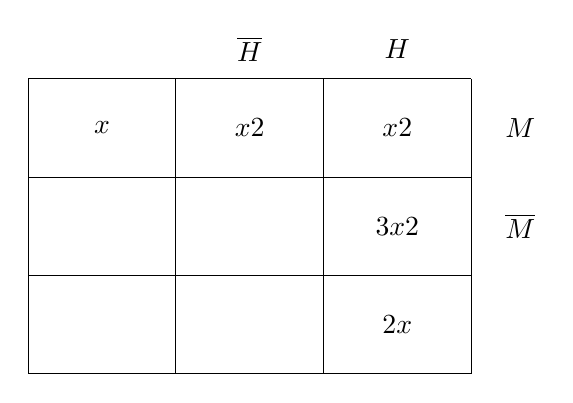
\begin{tikzpicture}[scale=1.25]
\draw (0,0) grid[xstep=1.5] (4.5,3);
\node at (3.75,3.3) {$H$};
\node at (2.25,3.3) {$\overline{H}$};
\node at (5,2.5) {$M$};
\node at (5,1.5) {$\overline{M}$};

\node at (3.75,2.5) {$\disfrac{x}{2}$};
\node at (2.25,2.5) {$\disfrac{x}{2}$};
\node at (0.75,2.5) {$x$};

\node at (3.75,1.5) {$\disfrac{3x}{2}$};
\node at (2.25,1.5) {$$};
\node at (0.75,1.5) {$$};

\node at (0.75,0.5) {$$};
\node at (2.25,0.5) {$$};
\node at (3.75,0.5) {$2x$};
\end{tikzpicture}
\end{center}

\textbf{סעיף ב 2}

במילה "לפחות" מכוונת לנוסחת ברנולי. נסמן
$p=P(H\cap M)$
ונחשב:
\begin{eqn}
P(p\geq 3) = P(p=3 \cup p=4)&=& {4\choose 3}p^3(1-p)^1+{4\choose 4}p^4(1-p)^0\\[6pt]
&=&4\cdot 0.0009 + 0.0001 = 0.0037\,.
\end{eqn}

%%%%%%%%%%%%%%%%%%%%%%%%%%%%%%%%%%%%%%%%%%%%%%%%%%%%%%%%%

\newpage

\section{חורף תשפ"א מועד נבצרים}

\begin{center}
\selectlanguage{english}
\includegraphics[width=\textwidth]{winter-2021nv-3}
\end{center}

נסמן ב-%
$M$ \L{(muzika)}
את המאורע של צופים במוזיקה ונסמן ב-%
$S$ \L{(sport)}
את המאורע של צופים בספורט. השאלה שואלת על שני סוגים של מאורעות ולכן נארגן את המידע בטבלה.

מהנתון הראשון ניתן לחשב את
$P(M)$:
\begin{eqn}
P(M)&=&1.5P(\overline{M})=1.5 (1-P(M))\\
P(M)&=&3/5\,.
\end{eqn}
בשני המשפטים הבאים, "מן הלקוחות" מכוון להסתברות מותנית:
\begin{eqn}
P(M/S)&=&\frac{P(M\cap S)}{P(S)}=2/3\\[4pt]
P(M\cap S)&=&(2/3)P(S)\\[4pt]
P(M/\overline{S})&=&\frac{(M\cap \overline{S})}{P(\overline{S})}=2/5\\[4pt]
P(M\cap \overline{S})&=&(3/5)P(\overline{S})\,.
\end{eqn}
נשתמש בהסתברות שלמה כדי לחשב את 
$P(S)$:
\begin{eqn}
P(M)&=&P(M\cap S)+P(M\cap \overline{S})=3/5\\
&=&(2/3)P(S)+(2/5)P(\overline{S})=3/5\\
P(S)&=&3/4\,.
\end{eqn}
לאחר שנחשב את
$P(M\cap S)$
ו-%
$P(M\cap \overline{S})$
מ-%
$P(S)$,
נוכל למלא אתת הטבלה:
\begin{center}
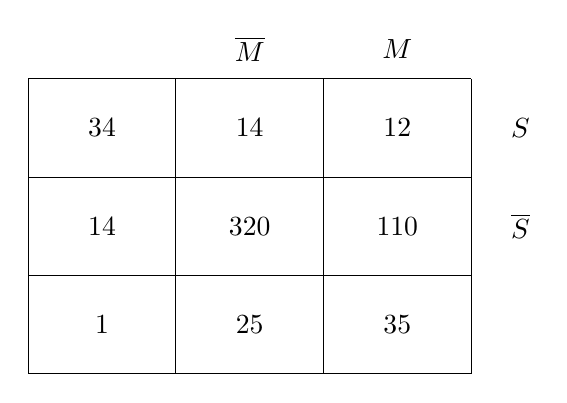
\begin{tikzpicture}[scale=1.25]
\draw (0,0) grid[xstep=1.5] (4.5,3);
\node at (3.75,3.3) {$M$};
\node at (2.25,3.3) {$\overline{M}$};
\node at (5,2.5) {$S$};
\node at (5,1.5) {$\overline{S}$};

\node at (3.75,2.5) {$\disfrac{1}{2}$};
\node at (2.25,2.5) {$\disfrac{1}{4}$};
\node at (0.75,2.5) {$\disfrac{3}{4}$};

\node at (3.75,1.5) {$\disfrac{1}{10}$};
\node at (2.25,1.5) {$\disfrac{3}{20}$};
\node at (0.75,1.5) {$\disfrac{1}{4}$};

\node at (0.75,0.5) {$1$};
\node at (2.25,0.5) {$\disfrac{2}{5}$};
\node at (3.75,0.5) {$\disfrac{3}{5}$};
\end{tikzpicture}
\end{center}

\textbf{סעיף א}

התשובה נמצאת בתא 
$P(M\cap S)=1/2$.

\textbf{סעיף ב}

המילא "או" מכוון לאיחוד של שני מאורעות. בעזרת תרשים
\L{Venn}
נקבל:
\[
P(M\cup S)=P(M)+P(S)-P(M\cap S)=\frac{3}{5}+\frac{3}{4}-\frac{1}{2}=\frac{17}{20}\,.
\]
ההמשך בהסתברות מותנית. הניסוח לא שגרתי אבל לא קשה: "נמצא שלקוח שנבחר ... מה ההסתברות 
\textbf{שהוא}":
\[
P(\overline{M}/M\cup S)=\frac{P(\overline{M}\cap (M\cup S))}{P(M\cup S)}=\frac{P(S\cap \overline{M})}{P(M\cup S)}=\frac{1/4}{17/20}=5/17\,.
\]
ברור ש-%
$M\cap\overline{M}$
היא הקבוצה הריקה ולכן
$\overline{M}\cap (M\cup S))=S\cap \overline{M}$.

\textbf{סעיף ג}

מהמידע בטבלה נחשב את ההסתברות שלבחור לקוח אחד כנדרש:
\begin{eqn}
P(M/\overline{S})&=&\frac{P(M\cap\overline{S})}{P(S)}=\frac{1/10}{3/4}=\frac{2}{5}\,.
\end{eqn}
"לפחות שניים" מכוון להתפלגות בינום, ונעדיף לחשב את ההסתברות המשלימה:
\begin{eqn}
P(M/\overline{S}\geq 2)&=&1-P(M/\overline{S}<2)\\[6pt]
&=&1-{4\choose 0}\left(\frac{2}{5}\right)^0\left(\frac{3}{5}\right)^4-{4\choose 1}\left(\frac{2}{5}\right)^1\left(\frac{3}{5}\right)^3\\
&=&\frac{328}{625}=0.5248\,.
\end{eqn}

%%%%%%%%%%%%%%%%%%%%%%%%%%%%%%%%%%%%%%%%%%%%%%%%%%%%%%%%%

\newpage

\section{חורף תשפ"א מועד מאוחר}

\begin{center}
\selectlanguage{english}
\includegraphics[width=\textwidth]{winter-2021lt-3}
\end{center}

נסמן ב-%
$A$ \L{(adom)}, $T$ \L{(tzahov)}, $K$ \L{(kakhol)}
את המאורעות של הוצאת כדורים אדומים, צהובים וכחולים, בהתאמה. נתון
$P(A)=5/8$, $3P(T)=P(K)$.
נסמן
$x=P(K)$
ונסכם הסתברויות כדי לקבל את המשוואה
\[
5/8+3x+x=1\,,
\]
שפתרונה הוא
$x=3/32$.
נארגן את המידע בטבלה.
\begin{center}
\selectlanguage{english}
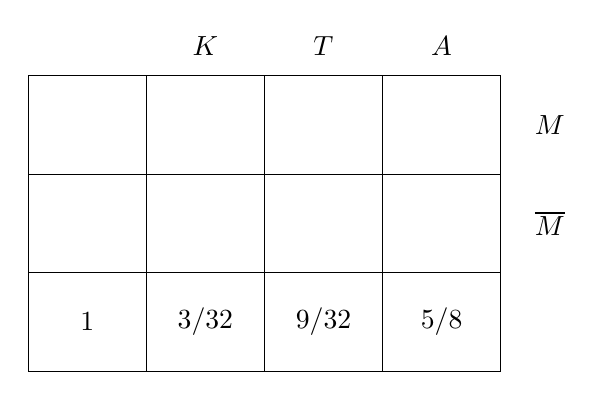
\begin{tikzpicture}[scale=1.25]
\draw (0,0) grid[xstep=1.2cm] (4.8,3);
\node at (4.2,3.3) {$A$};
\node at (3,3.3) {$T$};
\node at (1.8,3.3) {$K$};
\node at (5.3,2.5) {$M$};
\node at (5.3,1.5) {$\overline{M}$};

\node at (4.2,2.5) {$$};
\node at (3,2.5) {$$};
\node at (1.8,2.5) {$$};
\node at (0.6,2.5) {$$};

\node at (4.2,1.5) {$$};
\node at (3,1.5) {$$};
\node at (1.8,1.5) {$$};
\node at (0.6,1.5) {$$};

\node at (4.2,0.5) {$5/8$};
\node at (3,0.5) {$9/32$};
\node at (1.8,0.5) {$3/32$};
\node at (0.6,0.5) {$1$};
\end{tikzpicture}
\end{center}
נסמן ב-%
$M$ \L{(mekhuspas)}
את האירוע של כדור מחוספס. נתון:
\begin{eqn}
P(M\cap A)&=&\frac{4}{5}\,P(A)=\frac{1}{2}\\[6pt]
P(M\cap T)&=&\frac{8}{9}\,P(T)=\frac{1}{4}\,.
\end{eqn}
תחילה נראה לי שחסר נתון כדי להמשיך עד שקראתי בעיון את השאלה. הפסקה "כל שאר הכדורים חלקים" אומר ש-%
$P(M\cap K)=0$
וניתן למלא את כל התאים בטבלה עם הסתברויות משלימות:
\begin{center}
\selectlanguage{english}
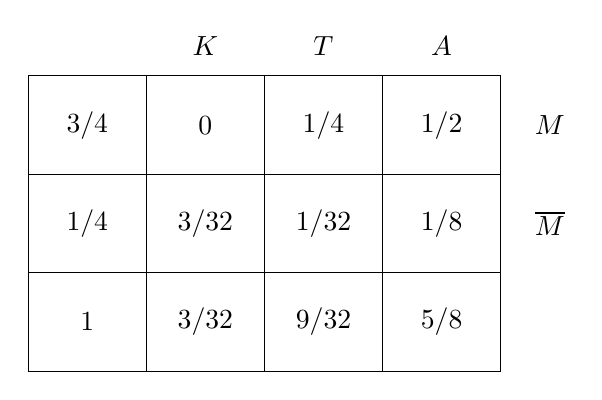
\begin{tikzpicture}[scale=1.25]
\draw (0,0) grid[xstep=1.2cm] (4.8,3);
\node at (4.2,3.3) {$A$};
\node at (3,3.3) {$T$};
\node at (1.8,3.3) {$K$};
\node at (5.3,2.5) {$M$};
\node at (5.3,1.5) {$\overline{M}$};

\node at (4.2,2.5) {$1/2$};
\node at (3,2.5) {$1/4$};
\node at (1.8,2.5) {$0$};
\node at (0.6,2.5) {$3/4$};

\node at (4.2,1.5) {$1/8$};
\node at (3,1.5) {$1/32$};
\node at (1.8,1.5) {$3/32$};
\node at (0.6,1.5) {$1/4$};

\node at (4.2,0.5) {$5/8$};
\node at (3,0.5) {$9/32$};
\node at (1.8,0.5) {$3/32$};
\node at (0.6,0.5) {$1$};
\end{tikzpicture}
\end{center}

\textbf{סעיף א}

"בדיוק" מכוון לנוסחת ברנולי. ההסתברות היא:
\[
P(M=3)={8\choose 3}\left(\frac{3}{4}\right)^3
\left(\frac{1}{4}\right)^5=56\cdot\frac{27}{65536}=\frac{189}{8192}=0.0231\,.
\]

\textbf{סעיף ב 1}

השליפות הן אחת אחרי השנייה ולכן נארגן את המידע בעץ, כאשר בכל שלב אפשר לשלוף כדור בצבע מסויים. השליפה היא ללא החזרה ולכן ההסתברויות שונות בשליפה הראשונה והשנייה.
\begin{center}
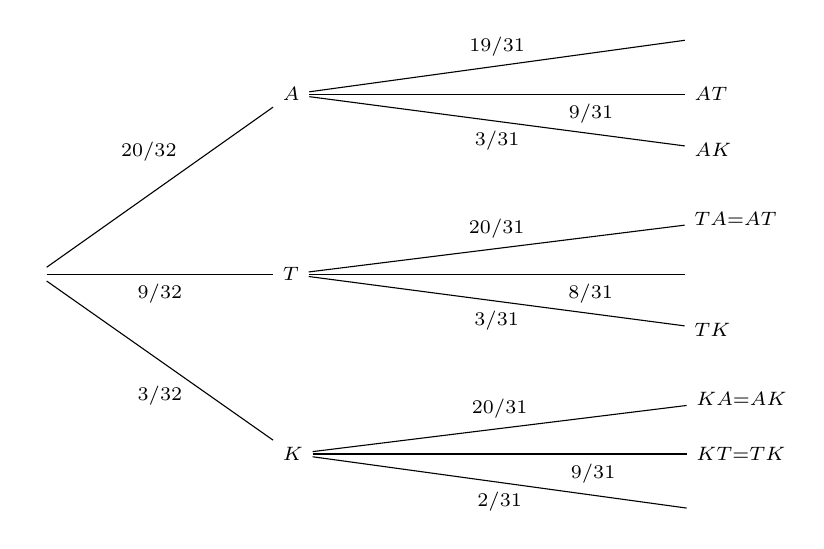
\begin{tikzpicture}
[grow=right,
level 1/.append style={level distance=3cm,
                       sibling distance=6.5em},
level 2/.append style={level distance=5cm,
                       sibling distance=2em}]
\node[left] {} % root
child {
  node[right] {$\scriptstyle K$}
    child {
      node[right] {}
      edge from parent node[below] {$\scriptstyle 2/31$}
    }
    child {
      node[right] {$\scriptstyle KT=TK$}
      edge from parent node[below,near end] {$\scriptstyle 9/31$}
    }
    child {
      node[right] {$\scriptstyle KA=AK$}
      edge from parent node[above] {$\scriptstyle 20/31$}
    }
    edge from parent node[below,yshift=-2mm] 
     {$\scriptstyle 3/32$}
}
child {
  node[right] {$\scriptstyle T$}
    child {
      node[right] {$\scriptstyle TK$}
      edge from parent node[below] {$\scriptstyle 3/31$}
    }
    child {
      node[right] {}
      edge from parent node[below,near end] {$\scriptstyle 8/31$}
    }
    child {
      node[right] {$\scriptstyle TA=AT$}
      edge from parent node[above] {$\scriptstyle 20/31$}
    }
    edge from parent node[below] {$\scriptstyle 9/32$}
}
child {
  node[right] {$\scriptstyle A$}
    child {
      node[right] {$\scriptstyle AK$}
      edge from parent node[below] {$\scriptstyle 3/31$}
    }
    child {
      node[right] {$\scriptstyle AT$}
      edge from parent node[below,near end] {$\scriptstyle 9/31$}
    }
    child {
      node[right] {}
      edge from parent node[above] {$\scriptstyle 19/31$}
    }
    edge from parent node[above,yshift=2mm,xshift=-4pt]
      {$\scriptstyle 20/32$}
}
;
\end{tikzpicture}
\end{center}
נסמן ב-%
$S$ \L{(shoneh)}
את המאורע שהכדורים בצבעים שונים:
\begin{eqn}
P(S)=P(AT\cup AK \cup TK)&=&
\frac{1}{32\cdot 31}
(2\cdot 20\cdot 9 + 2\cdot 20\cdot 3 + 2\cdot 3\cdot 9))\\[6pt]
&=&\frac{534}{992}=0.5383\,.
\end{eqn}
בדיעבד היה קל יותר לחשב את ההסתברות המשלימה לשליפת שני כדורים מאותו צבע!

\textbf{סעיף ב 2}

נסמן ב-%
$A_1$
את המאורע שהכדור הראשון בצבע אדום. "ידוע" מכוון להסתברות מותנית:
\begin{eqn}
P(A_1/S)&=&\frac{P(A_1\cap S)}{P(S)}=\frac{P(AT\cup AK)}{P(S)}\\[12pt]
&=&
\disfrac{
\disfrac{20\cdot 9 +  20\cdot 3}{32\cdot 31\rule[-5pt]{0pt}{5pt}}
}{
\disfrac{\rule[5pt]{0pt}{5pt}534}{32\cdot 31}
}=\frac{40}{89}=0.4494\,.
\end{eqn}

\textbf{סעיף ג}

$P(K)=3/32$
ולכן מספר הכדורים הכחולים הוא
$3n/32$.
בהנחה הברורה שיש מספר שלם של כדורים כחולים, הערכים ההאפשריים של 
$n$
הם
$32, 64, 96, 128,\ldots$.
בטווח הנתון האפשריויות הם
$64, 96$.